%&LaTeX
\batchmode
\documentclass{article}
%\usepackage{setspace}
\usepackage{graphicx}
%\usepackage{amsmath}
\usepackage{hyperref}
\usepackage{a4wide}
\def\R2Lurl#1#2{\mbox{\href{#1}{\tt #2}}}

\newcommand{\tab}{\hspace{5mm}}


\begin{document}
\begin{center}
\textbf{{\huge STIR \\
Overview for developers}}\\
\textbf{Kris Thielemans}\\
\textbf{\textit{version 3.1}}


\end{center}

\tableofcontents


\section{
Introduction}

The objective of this document is to describe the STIR common 
building blocks library.\\
The library has been designed so that it can be used for many 
different algorithms and scanner geometries, including both cylindrical 
PET scanners and dual-head rotating coincidence gamma cameras 
(although the latter needs some work). The library contains classes 
and functions to run parts of the reconstruction in parallel 
on distributed memory architectures, but the parallel features 
are not discussed here.\\
The building block classes discussed in this document are:
\begin{itemize}
\item
Classes for images (2D and 3D)
\item 
Classes for projection data (i.e. the measured data)
\item 
Forward projection, back projection and projection matrix classes.
\item 
Classes for iterative reconstruction algorithms
\item IO
\end{itemize}

The documentation
for the STIR library is generated automatically from the source 
using the \textit{doxygen} program (\R2Lurl{http://www.doxygen.org/ }{http://www.doxygen.org/}). 
This can produce an HTML version but also various other output 
formats (you can get e.g. RTF or LaTeX output by simply running 
doxygen on the source files that come in the STIR distribution). 


\section{
General conventions}



\subsection{
Units }

Distances are in millimetre.\\
Angles are in radians.\\
Relative times are in seconds.

\subsection{
Coordinate system for image data }

Although STIR is prepared for general images such as blobs on 
bcc grids (see the online documentation for class \textbf{DiscretisedDensity}), 
currently only voxels on a Cartesian grid are implemented (class \textbf{VoxelsOnCartesianGrid}). 
The coordinate axes for Cartesian grids are chosen as follows.
\begin{description}
\item[x-axis] : horizontal axis, pointing right when looking from 
the bed into the gantry
\item[y-axis] : vertical axis, pointing downwards
\item[z-axis] : the scanner axis, pointing from the gantry towards 
the bed
\end{description}
The origin of the X and Y axes are located on the central axis 
of the PET scanner and the Z origin (z=0) is located in the middle 
of the first ring (i.e at the opposite side of the bed). Note 
that for images with an even size in x and y, the axis of the 
scanner \textit{does} coincide with the centre of a pixel. In particular, 
for range of \textit{2n}, the (internal) image coordinates would run 
from \textit{-n} to \textit{(n-1)}.



\subsection{
Info on projection data}

Conventional axes and units used for projection data are shown 
in Figures \ref{scanner-image-units} and \ref{image-units}..

\begin{figure}[htbp]
\begin{center}
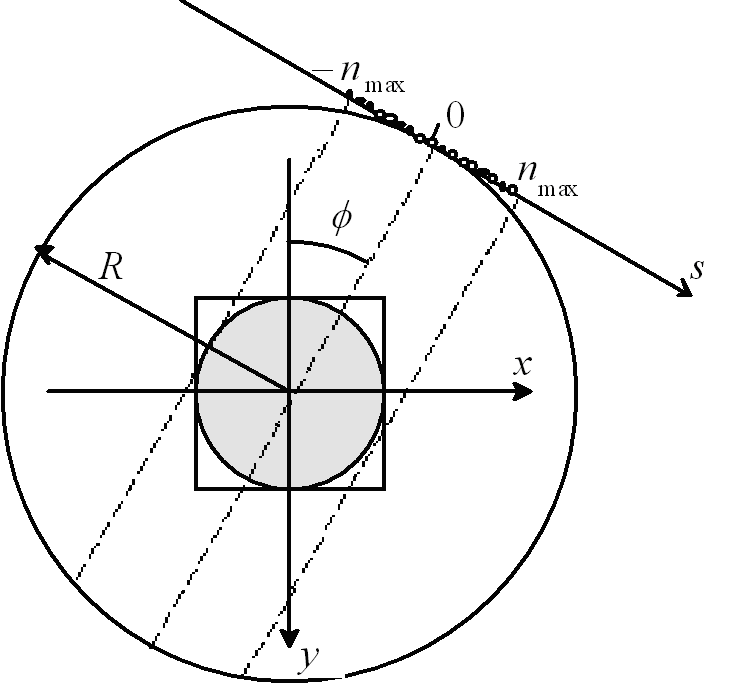
\includegraphics[width=2in, height=2in]{graphics/STIR-developers-overviewFig1}
\caption{ Axes and units within one transaxial 
slice of the target image. The transaxial section of the field 
of view is shown as a grey circle. The number of measured projection 
elements along the s-axis is odd, so that s =0 is positioned 
at the centre of the central projection element. The angles \ensuremath{\theta} 
and \ensuremath{\phi} define the direction of the line-of-response }
\label{image-units}
\end{center}
\end{figure}

\begin{figure}[htbp]
\begin{center}
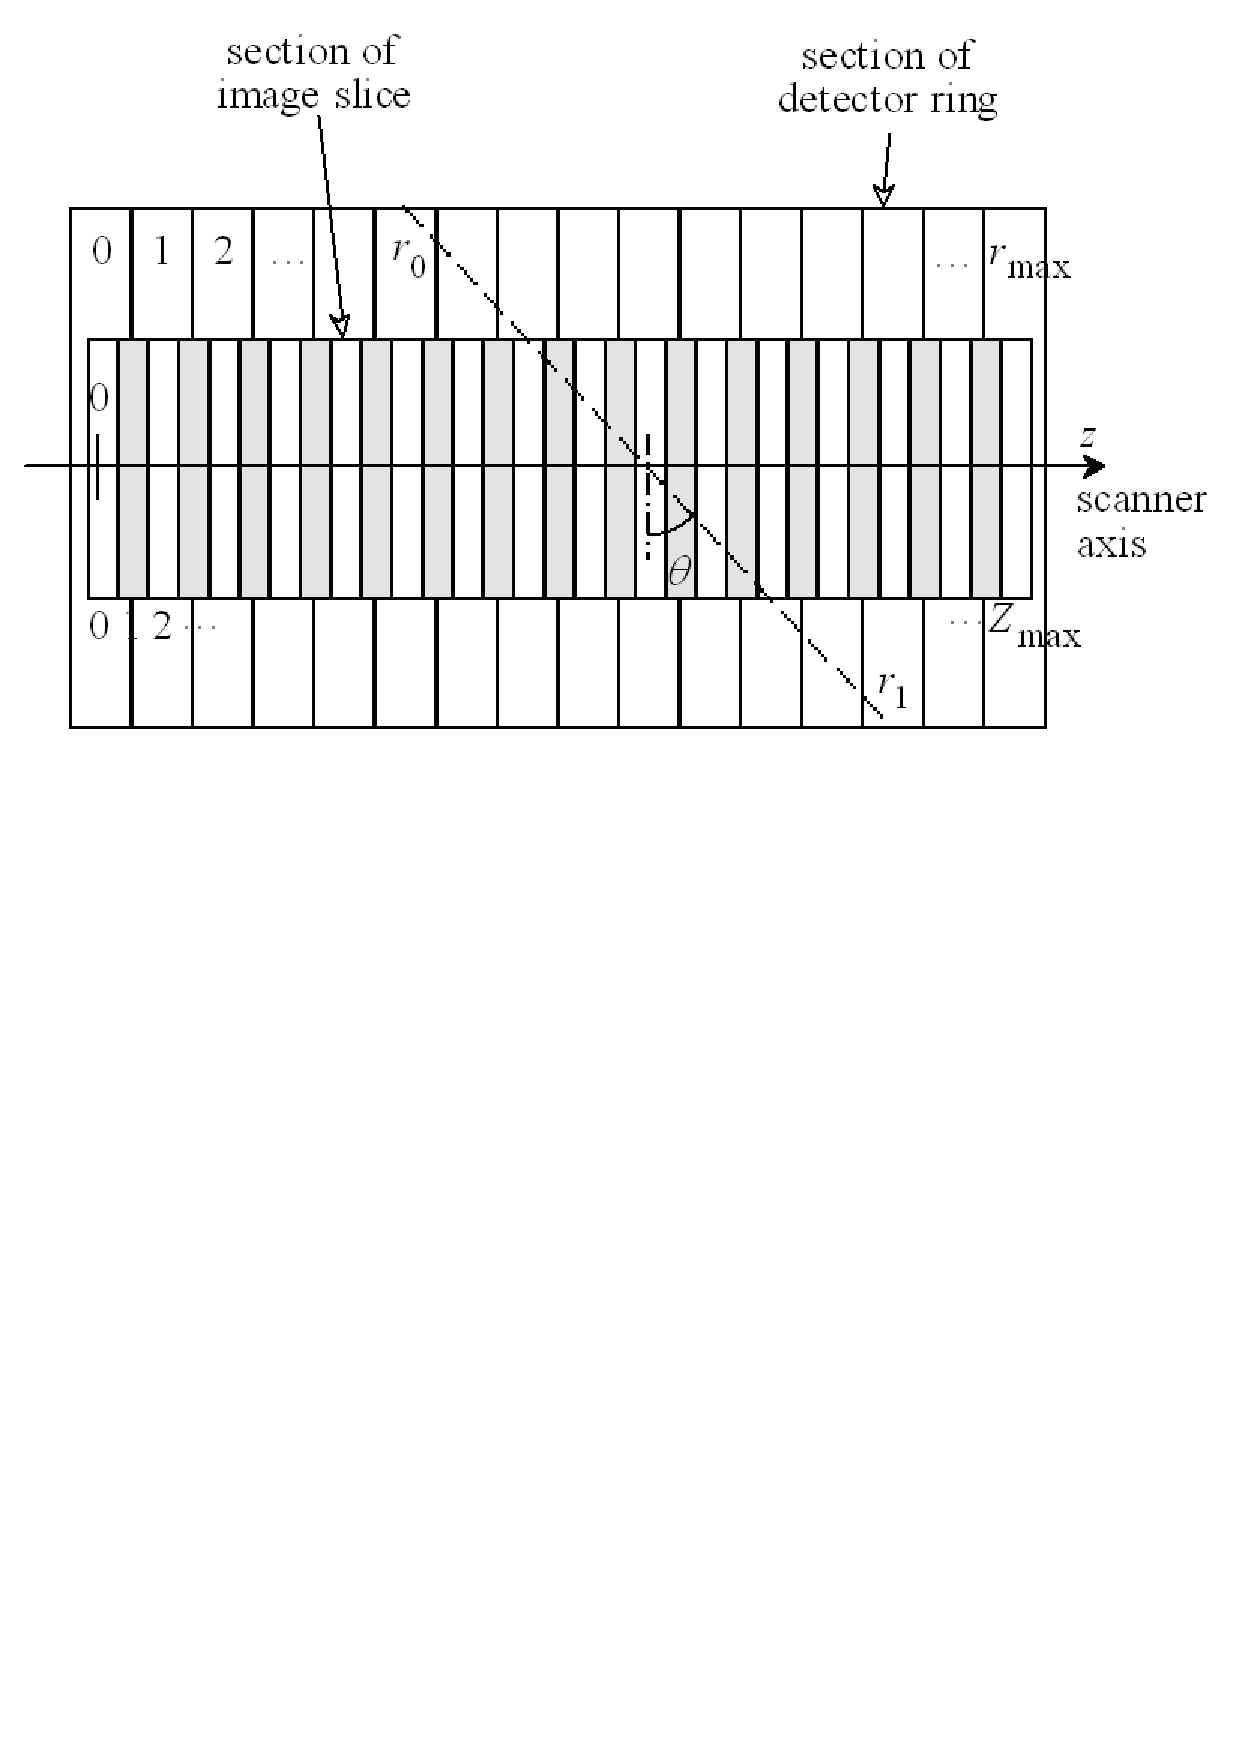
\includegraphics[width=4in, height=2in]{graphics/STIR-developers-overviewFig2}
\caption{Sketch of main axes, units and angles used in the cylindrical 
scanner geometry (axial section, not to scale)}
\label{scanner-image-units}
\end{center}
\end{figure}


See the STIR glossary for some info on naming conventions for 
projection data.


In 3D PET, two data storage modes are generally used for a \textbf{segment}\footnote{{The 
GE Advance file format does \textit{not} store the data per segment, 
but per view. In addition, the segments are then mixed. However, 
once read into STIR, this organisation is no longer available. 
\\
The ECAT6 sinograms also have no easy way to understand which 
ring-pair corresponds to which sinogram number for 3D PET. This 
is the main reason why STIR does not attempt to read ECAT6 sinograms 
directly, but leaves this to a separate conversion utility.}}
\begin{itemize}
\item 
where the 3D data is ordered by \textbf{sinogram} (i.e \textbf{axial position}, \textbf{view 
angle}, \textbf{tangential position}) (CTI terminology: \textit{Volume} mode) 
(see Figure \ref{fig:sinogramstorage})
\item where the 3D dataset is ordered by \textbf{view} (i.e \textbf{view angle}, \textbf{axial 
position}, \textbf{tangential position}) (CTI terminology: \textit{View}  
mode) (see Figure \ref{fig:viewgramstorage})
\end{itemize}

This notation means that for a sinogram, the tangential position 
runs fastest.\\
In both modes, the 3D dataset has been stored in several segments 
where the number of axial positions in each \textbf{segment} depends 
on the \textbf{axial compression (span)}.\\
Note that we find the CTI terminology confusing, so you will 
see it nowhere in STIR except in this document.


From both modes, 2 different types of 2D datasets can be obtained 
:
\begin{itemize}
\item Sinogram i.e (View, tangential position) for a fixed axial 
position.
\item Viewgram i.e (axial position, tangential position) for a fixed 
view.
\end{itemize} 


\begin{figure}[htbp]
\begin{center}
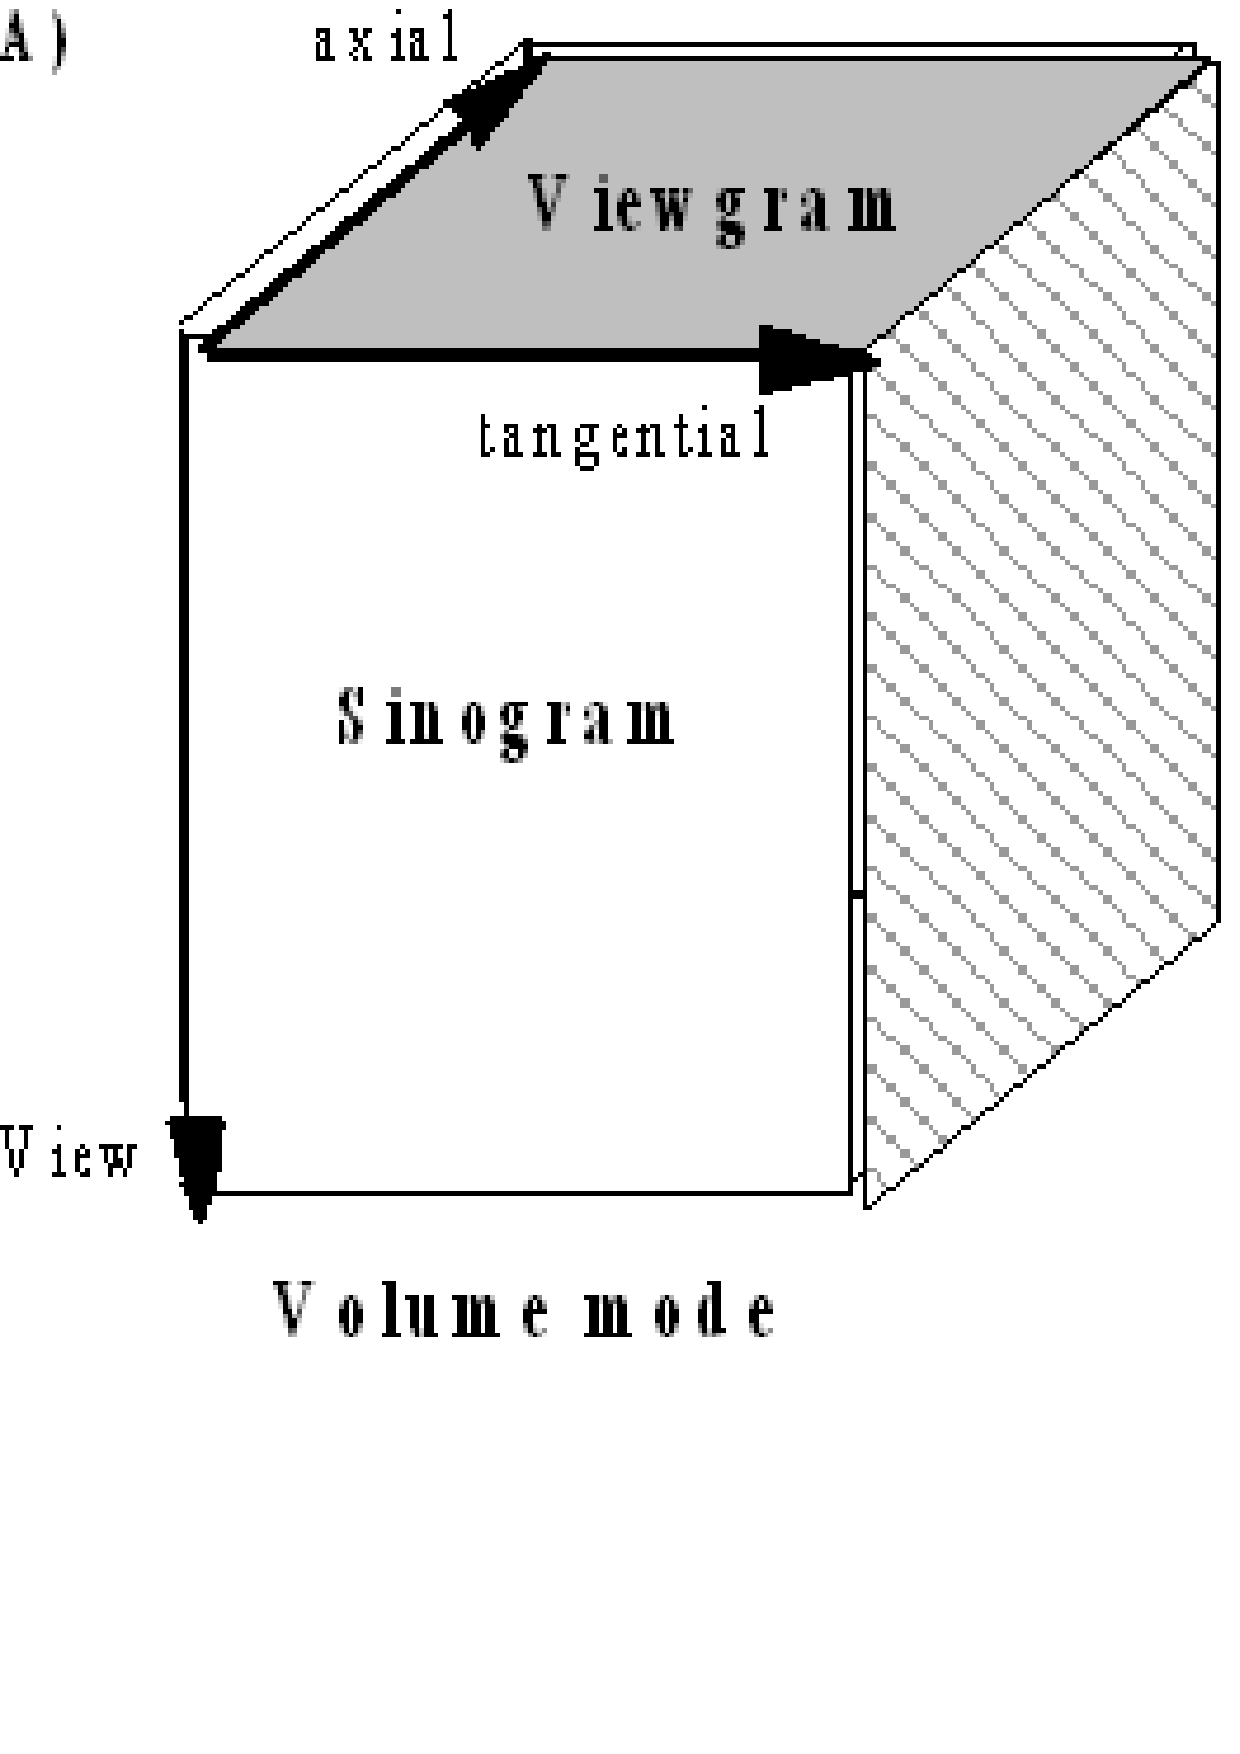
\includegraphics[width=2.7in, height=2.7in]{graphics/STIR-developers-overviewFig3}
\caption{By sinogram storage.}
\label{fig:sinogramstorage}
\end{center}
\end{figure}

\begin{figure}[htbp]
\begin{center}
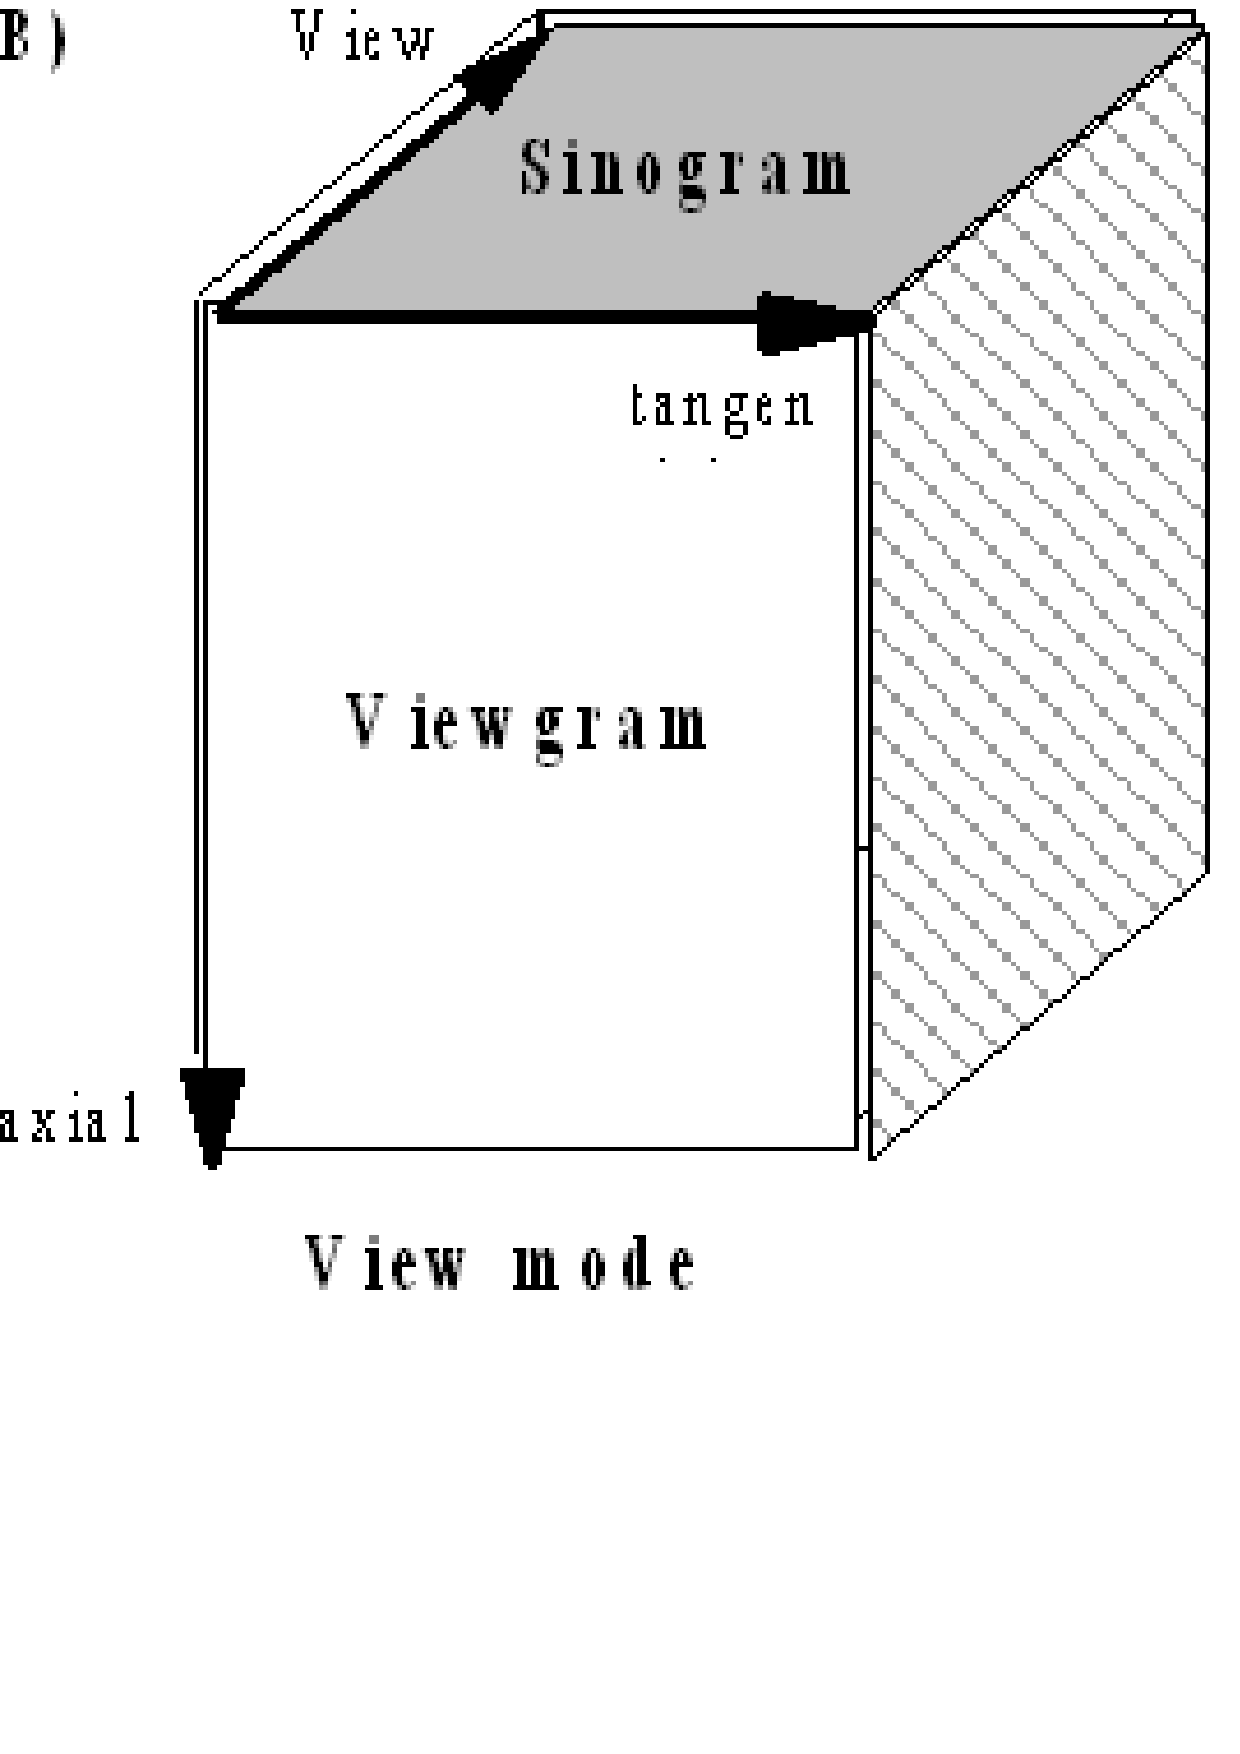
\includegraphics[width=2.7in, height=2.7in]{graphics/STIR-developers-overviewFig4}
\caption{By viewgram storage.}
\label{fig:viewgramstorage}
\end{center}
\end{figure}


For an \textit{N} ring scanner, if there is \textit{no} axial compression, 
there are \textit{N-abs(segment\_num)}  sinograms (or axial positions) 
in each segment. The first sinogram always corresponds to a coincidence 
in the first ring of the scanner (ring\_num=0), where the other 
ring would obviously be \textit{ring\_num=abs(ring\_diff)=abs(segment\_num)}. 
\\
Well ok, this is really true unless you messed around with the 
data and removed/added some sinograms. 

The situation with axial compression is more complicated. 
Obviously there is more than 1 ring-difference in a segment now. 
This makes it kind of hard to count how many sinograms/axial\_positions 
you will have and which ring-pairs sit in which segment. You 
can find some documentation on how we do this in ProjDataInfoCylindrical.cxx. 
See also the Michelogram documentation in the STIR glossary document. 


In any case, currently STIR always assumes for each segment that 
the middle of the scanner corresponds to the middle of the set 
of sinograms (taking into account the ring difference). 

View 0 currently corresponds to a vertical projection (for some 
scanners, this is not true. STIR currently ignores this, so will 
reconstruct a rotated image). Finally, in STIR code, the first 
ring of the scanner is the ring furthest from the bed. This corresponds 
to how the data are stored in ECAT6,7 and Interfile files.

\section{
Code conventions}


\subsection{
Configuration file}

The file \textit{stir}/\textit{common.h} contains general configuration 
info and tries to iron out some incompatibilities for certain 
compilers. If you include any STIR \textit{.h} file, you are guaranteed 
to have included \textit{stir}/\textit{common.h} as well, hence it should 
never be included explicitly by a 'user'.

\subsection{
Namespace}

The STIR library has its own C++ namespace: \textit{stir}. All symbols 
are within this namespace. The effect of this is that conflicts 
with other symbols are impossible (except when somebody else 
is using the same namespace). STIR also uses sub-namespaces for 
certain things. This usage will probably be expanded in the future.\\
For older compilers, the namespace can be disabled (see \textit{stir}/\textit{common.h}). 
For this reason, we have introduced some macros such as \textit{START\_NAMESPACE\_STIR.} You 
could use the macros in your own code as well, although people 
with a compiler that does not support namespace really should 
upgrade.

\subsection{
Naming conventions }

Types start with capitals, every word is capitalised, no underscores, 
e.g. \textit{DiscretisedDensity}.\\
Variables, methods and members are lower case, underscores between 
different words, e.g. \textit{voxel\_size}.\\
Variables, methods and members indicating 
\begin{itemize}
\item 
a variable or member used to indicate the number of things starts 
with \textit{num}, e.g. \textit{num\_gates}.
\item 
the number of an item in a sequence end with \textit{num}, e.g. \textit{gate\_num}.
\item 
a relative time (normally with respect to the scan start) end 
with \textit{rel\_time}, e.g. \textit{tracer\_injection\_rel\_time}.
\item 
Pointers to an object called \textit{something\_ptr}. Currently there 
is no naming distinction between shared pointers etc. This is 
probably a bad idea. For new code, we recommend to use \textit{something\_sptr} 
for shared pointers, and \textit{something\_aptr} for auto\_ptrs (see 
section \ref{sect:sharedptr}).
\end{itemize}

In most cases, access to data of a class is via a \textit{get\_something(), 
set\_something()} pair.\\
In general, names are descriptive and hence long. We often take 
longer to decide about the name than to write the actual code. 
If you write new code, do the same. You will be grateful when 
you look back at the code a few months later (and not vilified 
by your successor). 

\subsection{
File conventions }

Most classes have their own \textit{.h,} .\textit{inl}, \textit{.txx} and/or \textit{.cxx} files. 
File names of such classes are simply \textit{ClassName.h} {\nobreakspace}etc. 
(preserving capitals). In general, looking at 
the \textit{.h} file should give enough information on what a class/function 
does. \\
The \textit{.inl} files contain inline code 
for functions. The main purpose for this is to keep the \textit{.h} 
files as short and clean as possible. \\
The \textit{.txx} files are similar to the \textit{.inl} files. They contain non-inline 
definitions of template classes (or functions). They should only be included by the
corresponding \textit{.cxx} file where the template is then instantiated for any desired types.
This makes it easier or a user to instantiate a template for a new type without modifying the
original STIR code.\footnote{The \textit{.txx} extension as used because the Insight Toolkit (ITK) 
uses it as well. It stands for template C++ presumably.}


All STIR include files should be included as \textit{\#include ``stir/maybe\_a\_subdir/name.h''}\\
The \textit{doxygen} comments generally occur in the \textit{.h} file, unless 
they are very extensive. In this case, the \textit{.h} file contains 
a brief comment, while the \textit{.inl} or \textit{.cxx} file contains 
the longer description.\\
To avoid unnecessary interdependencies between \textit{.h} files (and 
hence unnecessary rebuilds when modifying one \textit{.h} file), we 
avoid including \textit{.h} files for 'supporting' classes as much 
as possible. Instead, we only declare the classes needed, e.g. \textit{class 
Bin;} instead of \textit{\#include stir/Bin.h.}



\subsection{
Class definitions}

Class definitions follow generally the following format (ignoring \textit{doxygen} 
comments).

\begin{verbatim}
class A
{
public: 
  enumerated types and other typedefs 
  static member functions  
  data members  
  constructors 
  destructors 
  member functions
protected: 
  enumerated types and other typedefs 
  static member functions 
  data members 
  constructors 
  destructors 
  member functions
private: 
  enumerated types and other typedefs 
  friends if any 
  static member functions 
  data members 
  constructors 
  destructors 
  member functions
};
\end{verbatim}


Inline member functions are defined in the \textit{.inl} file, and 
are ordered (where possible) such that if inline member function 
a() calls inline member function b(), 
then b should be defined first. (Otherwise very 
few compilers are able to inline the call to b 
from a.)



\subsection{
Argument order conventions}

When passing output arguments (by reference or by pointer), those 
arguments occur FIRST in the list. For instance
\begin{verbatim}
void some_function(int& output, const SomeType& some_input_argument, ...);
\end{verbatim}


This order of arguments allows the use of default arguments. 
Note that the standard C++ library does not use this convention.

\subsection{
Error handling }

Problem reporting is via two functions \textit{error()} and \textit{warning()}. 
Currently, \textit{error()} throws an exception. If you do not ``catch'' that
exception, the program will be simply aborted (after writing 
a diagnostic message). 

In many places, validity of input arguments or of the state of 
an object is checked by \textit{assert} macros. This code is only 
compiled when the \textit{NDEBUG} preprocessor macro is not defined (for isntance,
when setting \texttt{CMAKE\_BUILD\_TYPE} to \texttt{Debug}), 
such that a production version of the programs 
is not slowed down. If an assertion is false, the program aborts 
with info on the file and line number where the assertion failed.

\subsection{\label{ssect:AdvancedCppFeatures}
Advanced (?) C++ features used}

We attempted to follow the ANSI C++ standard as close as possible. 
We expect to have some marginal problems with a 'strict' ANSI 
C++ compiler, although there should now be very few cases (as 
gcc warns about a lot of stuff). We have used some preprocessor 
macros (see \textit{stir/common.h}) to isolate work-arounds for older 
compilers. Ideally, all these \#ifdefs should disappear at a 
later development stage of the library. We gradually give up 
on supporting older compilers anyway.


\subsubsection{Templates}
The library uses templates very often. This allows us to write 
'generic' code, independent of specific types. For instance, 
multi-dimensional arrays correspond to 

\begin{verbatim}
template <int num_dimensions, typename elemT>
class Array;
\end{verbatim}


To avoid linking problems, the templates which we use are explicitly 
instantiated in the relevant \textit{.cxx} files. If a user needs 
other types, (s)he will have to add the instantiations. In some cases,
this is not necessary as all methods of a template class are inlined, or the
actual definition is in a \textit{.txx} file that you can include.\\
We do use partial class template specialisation in some places. 
However, (very ugly) work-arounds are provided for compilers 
that do not support this feature (although not anymore in recent code).\\
Very occasionally we use member templates (in such a form that 
it could be compiled by Visual C++ 6.0, i.e. inline in the class definition). 

\subsubsection{Run Time Type Information}
Another C++ feature that we use is Run Time Type 
Information (RTTI). We almost exclusively use this to check validity 
of pointer (or reference) casts down a hierarchy ('down-casting'). 
See section \ref{sect:classhierarchies} 
for an example. If a compiler does not support 
RTTI (but all compilers do these days), it would be possible to declare 
a (essentially empty) \texttt{dynamic\_cast} 
template function such that the above code would compile. The 
resulting programme would become inherently type-unsafe though, 
and we recommend that you upgrade your compiler. Some code does 
rely on explicit type checking, you would have to check this 
in detail if you don't have RTTI.

\subsubsection{
Iterators}

An important C++ concept, used fairly often in STIR, is an \textit{iterator.} The 
easiest way to think about iterators is as a sort of generalised 
pointer, used to iterate through a collection of objects of the 
same type. For instance, the following code would add 2 to all 
the elements of a vector:

\begin{verbatim}
void f(vector<int>& v)
{
  for (vector<int>::iterator iter = v.begin(); iter != v.end(); ++iter)
     *iter += 2;
}
\end{verbatim}


So, just as pointers, you increment an iterator to go to the 
next element of the vector, and you use \textit{*iter} to access the 
object that the iterator refers to. However, the advantage is 
that the above code would just as well work for any other type 
of collection, as long as it provides an iterator interface. 
So, typical code in C++ would look as follows:

\begin{verbatim}
template <class Container>
void f(Container& v)
{
  for (typename Container::iterator iter = v.begin(); iter != v.end(); ++iter)
     *iter += 2;
}
\end{verbatim}


Iterators are used with great success in the C++ Standard Template 
Library (STL), and STIR provides iterators for its container 
classes. In particular, for multi-dimensional arrays, it is possible 
to iterate through the array in 2 ways: using \textit{Array\texttt{<}n,T\texttt{>}::iterator} 
whose iterators point to arrays of dimensions \textit{n-1}, or using \textit{Array\texttt{<}n,T\texttt{>}::full\_iterator} which 
essentially provides a one-dimensional look at the whole array. 
So, adding 2 to all the elements of a multi-dimensional array 
can be done as follows

\begin{verbatim}
template <int n, class elemT>
void f(Array<n,elemT>& a)
{
  for (typename Array<n,elemT>::full_iterator iter = a.begin_all(); 
       iter != a.end_all(); ++iter)
     *iter += 2;
}
\end{verbatim}

Note that use of the \textit{begin\_all()} and \textit{end\_all()} members 
which return \textit{full\_iterator} objects. \\
Of course, the above function is just an illustration, as in 
STIR this can be done by using:


\begin{verbatim}
Array<n,elemT> a = ...;
a += 2;
\end{verbatim}


\subsubsection{
Shared pointers and other smart pointers \label{sect:sharedptr}}

STIR uses the \texttt{shared\_ptr} class considerably. Shared pointers 
are a specific type of 'smart pointers'. These have the advantage 
that they essentially clean up after you. That is, you do not 
have to call \textit{delete} on them. They are even exception proof 
(something which you cannot achieve with an ordinary pointer). 
Generally, the destructor of the smart pointer will make sure 
that the object it points to is deleted (when appropriate).\\
\textit{std::auto\_ptr} is a standard smart pointer class which is 
suitable for pointers to objects where there's only one smart 
pointer for each object. Unfortunately, its syntax has been decided 
rather late in ANSI C++ and its implementation requires some 
advanced C++ features, leading to a non-standard implementation 
of \texttt{std::auto\_ptr} in older compilers (including VC 6.0) and it is now
superseded by \texttt{std::unique\_ptr} in C++11. For this 
reason, we do not use this smart pointer class too much, and 
generally use \texttt{shared\_ptr} instead. This is somewhat unfortunate 
as these two smart pointers are generally quite different concepts. 

\texttt{shared\_ptr} is a STIR (or boost) smart pointer class which 
is suitable when there are (potentially) more than one pointer 
pointing to the same object. It keeps a reference count such 
that the object is (only) deleted when the last shared pointer 
that references it is destructed. \\
\textbf{Caveat}: if you modify the object of 1 \texttt{shared\_ptr}, the change 
obviously applies to all shared\_ptrs sharing that object.\\
\textbf{Caveat}: if you assign an ordinary pointer to a \texttt{shared\_ptr}, you 
cannot delete the ordinary pointer anymore (it will be done by 
the \texttt{shared\_ptr}). As a consequence, you cannot assign an ordinary 
pointer twice to a \texttt{shared\_ptr}. It is thus better to go all the 
way, and not have any ordinary pointers anymore.\\
\textbf{Caveat}: do not initialise a \texttt{shared\_ptr} with a pointer that cannot/should 
not be deleted. For instance, initialising it with the address 
of a local variable, or even a reference, will cause a delete 
on an object that is not allocated on the heap, and so probably 
crash your program.

It is clear that smart pointers are very useful, but also somewhat 
dangerous. For this reason, most classes do not return shared\_ptrs 
to their members (even if they store one). Instead, they return 
a pointer to a const object. This prevents a user of a class 
to inadvertently change members of the class-object. This does 
involve a memory/performance penalty when the user then needs to create 
a \texttt{shared\_ptr} himself. For example, you'll see code like this

\begin{verbatim}
ProjData proj_data(...);
ProjDataInfo const * proj_data_info_ptr = 
  proj_data.get_proj_data_info_ptr();
shared_ptr<ProjDataInfo> new_proj_data_info_sptr(proj_data_info_ptr->clone());
// now do something with new_proj_data_info_sptr
\end{verbatim}


We provide the convenience function \textit{stir::is\_null\_ptr()} 
to test if a pointer is `null', i.e. does not point to anything. \textit{is\_null\_ptr} 
works with ordinary pointers, shared\_ptrs and auto\_ptrs. Use 
it to avoid that your code depends on what type of (smart) pointer 
you are using.

\subsection{Generic functionality of STIR classes}
This is a (very incomplete) section describing some functionality that
many STIR classes have in common.

\subsubsection{Copying objects}
When using pointers or references to objects of an abstract type, you can copy 
them using \texttt{clone()}, see section \ref{sect:sharedptr}.


When you only want to create an object of the same characteristics, but without
copying the data itself (e.g. images of the same size), use \texttt{get\_empty\_copy()}.

\subsubsection{Comparing objects}
Many STIR classes implement comparison using the usual \texttt{==} and 
\texttt{!=} operators. The implementation of these operators is somewhat 
tricky in class hierarchies. We try to follow the approach described in
\textit{Overriding the C++ Operator==, An approach that uses the 
Template Method design pattern} By Daniel E. Stevenson and Andrew T. Phillips,
Dr. Dobb's Journal, June 2003, 
\R2Lurl{http://www.ddj.com/184405409}{http://www.ddj.com/184405409}.

For some classes, you might want to check only if two objects are of the same
type. For instance, if images have the same sizes, origin etc, but not 
necessarily the same voxel values. This can be done using the member
function \texttt{has\_same\_characterics}.

\subsubsection{Parsing from text files}
Many class-hierarchies allow to construct an object by parsing a 
text file, which uses an Interfile-like syntax. Examples
are given in the User's guide. see section \ref{sect:parsing}.

All these classes (and some others) have a member function 
\texttt{parameter\_info()} which returns a string with all parameters
of the object.

Note that many STIR classes are not completely constructed by parsing.
Usually, it is necessary to call a \texttt{set\_up} function to make
the object usable.

\subsubsection{typedefs}
Many class hierarchies use the same typedefs. For example:
\begin{verbatim}
class ProjDataInfo
{
protected:
  typedef ProjDataInfo root_type; // root of hierarchy
  
};
class ProjDataInfoCylindrical: public ProjDataInfo
{
private:
  typedef ProjDataInfo base_type;
  typedef ProjDataInfoCylindrical self_type;
};
\end{verbatim}

\section{
Overview of classes}

This section provides an overview of the main ingredients of 
the library. Detailed description of these classes is in the documentation. 
Below we only mention some general features.



\subsection{
Images}

Iterative algorithms generally assume that the activity density 
can be discretised in some way. That is, the continuous density 
can be approximated by having a linear combination of some basis-functions. 
The reconstruction problem will try to estimate the coefficients $\lambda_{ijk}$ of 
the discretised density


$\sum_{ ijk}\lambda _{ijk} \,b_{ijk} (\widehat{x})  $

The base class corresponding to this kind of data is \textit{DiscretisedDensity.}\\
We assume that the set of basisfunctions can be characterised 
by 3 indices\footnote{{\small Actually most of the image hierarchy is 
templated in the number of dimensions. This means it can be used 
for 2D and 3D images, but also for higher dimensional cases (say 
temporal information).}} $(ijk)$ such that $i$ runs over a 
range of integers $i_1..i_2$,$j$ runs over a 
similar range that can however depend on $i$, and $k$ runs 
over a similar range that can depend on $i$ and $j$. 
This 
concept of ranges is embodied in the \textit{IndexRange} class. Multi-dimensional 
arrays which have such ranges are encoded by the \textit{Array} class. 
This forms the data structure for the set of coefficients of 
the basisfunctions, hence \textit{DiscretisedDensity} is derived from 
the \textit{Array}.


In most useful cases, the basisfunctions will be translations 
of a single function \textit{b(x)} (although scaling etc could occur 
depending on \textit{ijk)}. This means that the discretisation has 
a certain grid, corresponding to the centre of the basisfunctions. 
This structure is the next level in the image hierarchy. Currently 
we have the class \textit{DiscretisedDensityOnCartesianGrid} to implement 
the case where the grid is formed by an orthogonal set of vectors. 
Another case would be e.g. \textit{DiscretisedDensityOnCylindricalGrid} 
(for a cylindrical coordinate system), but we have not implemented 
this yet.\\
The next level in the hierarchy is then finally the specification 
of the basis functions themselves. We currently have only voxels 
and pixels, but another useful case would be to use Kaiser-Bessel 
functions as the translated basisfunction \textit{b(x)} (this is called \textit{Blobs} 
in the literature). This leads us to the example image hierarchy 
in Figure \ref{image-hierarchy}.\\
\begin{figure}[htbp]
\begin{center}
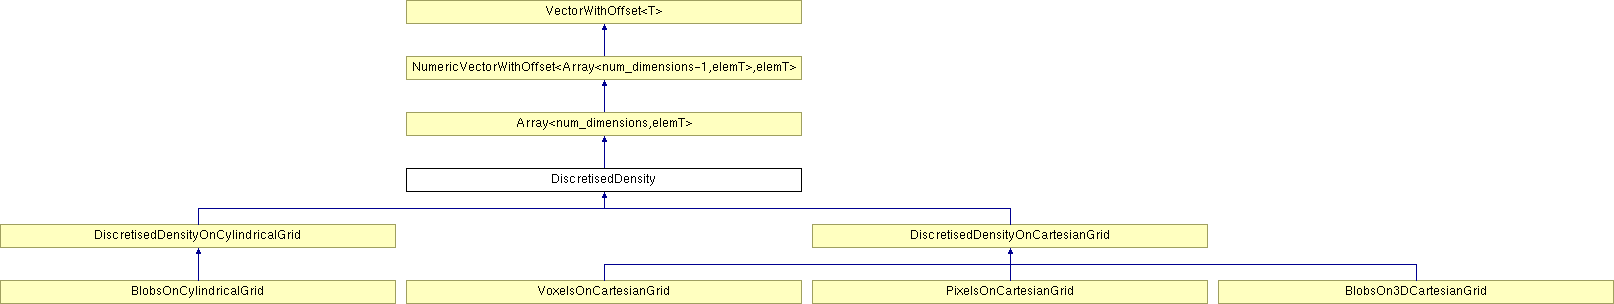
\includegraphics[bb = 0 0 1613 303, scale=0.25]{graphics/STIR-developers-overviewFig7}
\caption{ Hierarchy of classes for images. Only two 
of the bottom classes are currently implemented.}
\label{image-hierarchy}
\end{center}
\end{figure}


Although a Cartesian grid seems the logical choice for images, 
there are two reasons why one would like to use different types 
of grid. One important reason would be sampling efficiency. As 
an example, in 3D one needs less sampling points with a BCC grid 
while still being able to represent the same spatial frequencies. 
This becomes particularly important when using more complicated 
basis functions than voxels, like Kaiser-Bessel functions ('blobs'). 
In this case, calculations to perform the projections are much 
more expensive, so having less grid points becomes important. 
A second reason for changing the image grid is to increase the 
symmetry of the projection matrix. For example, for cylindrical 
scanners using a cylindrical grid would maximise the amount of 
repetition in the projection matrix. In particular, this would 
allow even for large PET scanners pre-calculation of the 'independent' 
part of the projection matrix, and loading it completely into 
memory when doing the reconstruction. This will not only speed 
up the reconstruction, but also enable more accurate models of 
the acquisition to be used, resulting in potentially better resolution 
and noise behaviour. We believe that this hierarchy can accommodate 
all known cases used for reconstructions in 3D PET.



\subsection{
Projection data classes}

Different manufacturers use different sampling of projection 
space. As an example, the HiDAC uses 'polar' sampling. Similarly, 
Single Photon Emission Tomography (SPET) or Computed Tomography 
(CT) data are very similar to PET. By having projection data 
classes that allow for different geometries and file formats, 
our library should be useful for these image modalities as well.\\
The general class to access projection data is called \textit{ProjData}. 
As in 3D-PET, the projection data are potentially huge, we do 
not generally store the whole data in memory. Instead, \textit{ProjData} 
has methods for getting subsets of the data, i.e. \textit{SegmentByView, 
SegmentBySinogram, Viewgram, Sinogram, RelatedViewgrams} (see section 
\ref{sect:sect:symmetries}). 
In addition, the \textit{ProjData} class provides access to a \textit{ProjDataInfo} 
object (see Figure \ref{projdatainfo-hierarchy}). This object completely describes the 
geometry of the data.

\begin{figure}[htbp]
\begin{center}
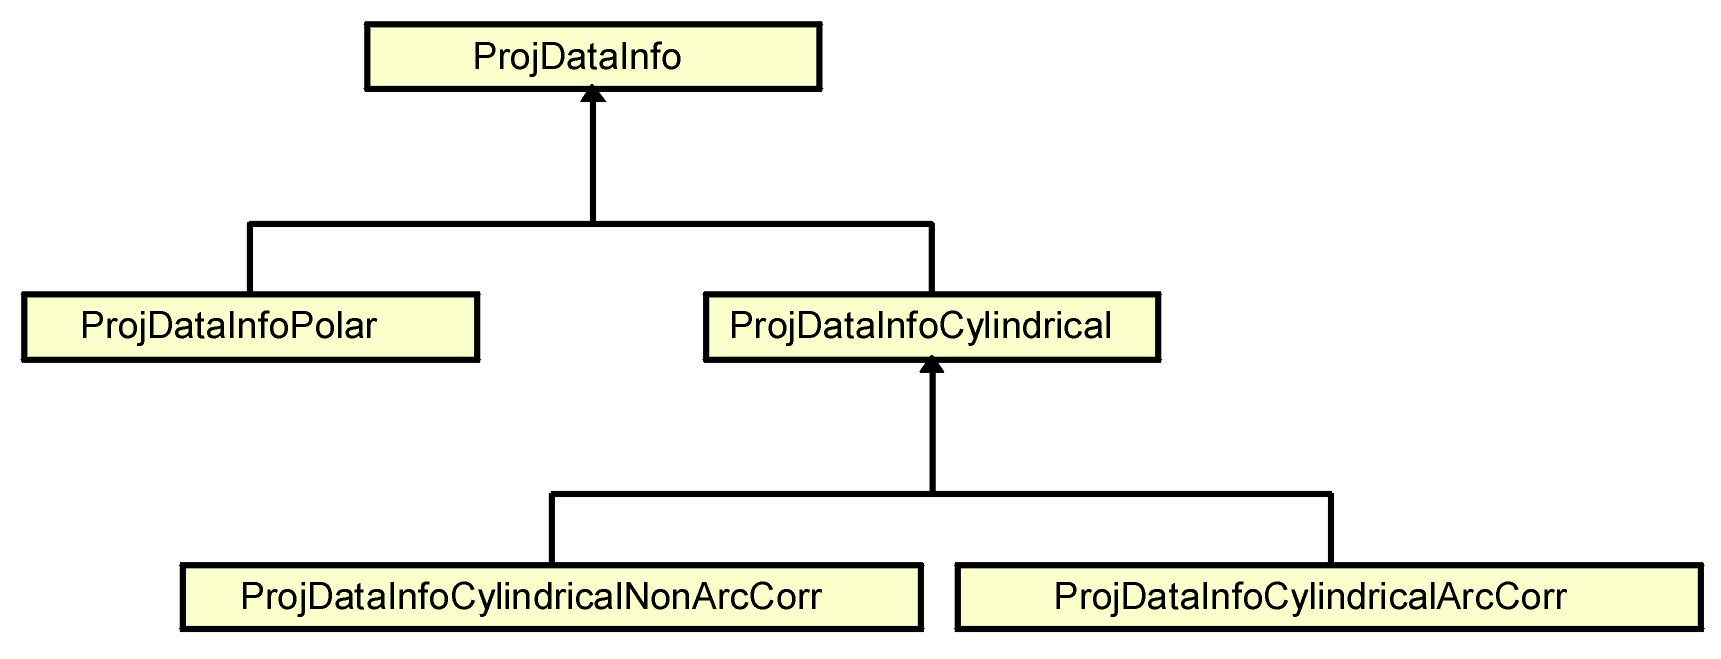
\includegraphics[width=4in, height=1.6in]{graphics/STIR-developers-overviewFig8}
\caption{ Hierarchy of classes for (geometric) information 
of the projection data.}
\label{projdatainfo-hierarchy}
\end{center}
\end{figure}


Different file formats (or potentially other types of projection 
data) are handled by having derived classes of \textit{ProjData}, 
which provide specific implementations for the data access methods. 
This hierarchy is at the moment very simple, but can easily be 
extended to accommodate different file formats.

\begin{figure}[htbp]
\begin{center}
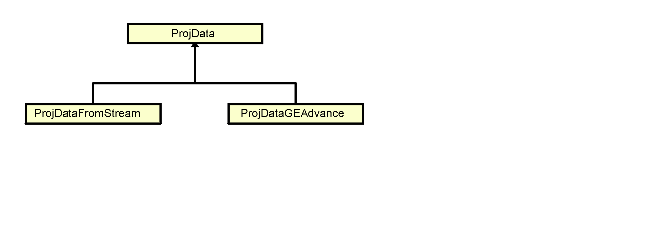
\includegraphics[width=5.103in, height=1.251in]{graphics/STIR-developers-overviewFig9}
\caption{ File formats for projection data}
\end{center}
\end{figure}


Currently missing is support for fan-beam data.\\
List-mode data is experimentally supported since version 1.2.

\subsection{
Data (or image) processor hierarchy}

We provide a hierarchy for functions that modify an image, \textit{e.g.} by 
filtering or thresholding it. The base class is \textit{DataProcessor},
which is templated in \texttt{DataT}, to allow using other types, not
only images.
Aside from the virtual functions that specify the interface to 
an image processor, it also provides the basics for a registry 
of all data processors. See section \ref{sect:registries} for some details.
Note that the registry is specific to every \texttt{DataT}.

\subsection{
Projector classes}

The next important type of ingredient for an iterative algorithm 
are the projection operations. The forward projection models 
the measurement. Generally, reconstruction algorithms are some 
kind of inversion procedure for the following problem


\[y_{b} =\sum\limits_{v}P_{bv} \lambda _{v}  \]


where $y_b$ are the measured data. The exact interpretation 
of the projection matrix depends on the algorithm (it is most 
of the time probabilistic, in the sense that the above equation 
would only hold 'on average' ). However, this need not concern 
us here.\\
Many algorithms (in particular EM-type algorithms) can be written 
solely in terms of multiplication with the projection matrix 
(\textit{forward projection}) or with its transpose (\textit{back projection}). 
This is why we have a \textit{ForwardProjectorByBin} and \textit{BackProjectorByBin} 
hierarchy. The basic objects handled by these projector classes 
are \textit{RelatedViewgrams} and (a derived class from) \textit{DiscretisedDensity}. 
Other algorithms (for instance ART or listmode algorithms) need 
more detailed access to the elements of the projection matrix, 
and hence will work with a \textit{ProjMatrixByBin} object\footnote{{\small Some 
algorithms would need column-wise access to the projection matrix 
(i.e. by voxels). We did not implement any of these algorithms, 
so we do not have appropriate projection classes for them. Modification 
of the row-wise classes is straightforward though.}}. 


\subsubsection{
Symmetries \label{sect:sect:symmetries}}

An important feature of geometric projectors is that several 
parts of the projection matrix are the same. This is because 
different (generalised) voxels and bins are related by symmetry. 
It is important to make use of these symmetries for two reasons. 
It allows storing only a part of the projection matrix (useful 
for disk storage and caching), and in on-the-fly projection operations 
it can be used to speed up the computation, as there is no need 
to recompute the related elements. As the number of projection 
data elements related by symmetry depends on the specific geometries 
(e.g which class derived from \textit{DiscretisedDensity} is used), 
we need classes (e.g. \textit{RelatedViewgrams}) that store all related 
data, classes for describing the symmetries (e.g. \textit{DataSymmetriesForViewSegmentNumbers}), 
and the necessary operations (\textit{SymmetryOperation}). \\
At the moment, the only symmetries implemented are specific for 
Cartesian grids. A discussion of these symmetries is presented 
in [Par4.1], but also in the online documentation.

\subsubsection{
ForwardProjectorByBin hierarchy}

We provide two derived classes of \textit{ForwardProjectorByBin}: 
\begin{itemize}
\item 
\textit{ForwardProjectorByBinUsingRayTracing} computes the $P_{bv}$ 
elements as the length of intersection of one Line Of Response 
with the voxel. The actual implementation uses a version of Siddon's 
algorithm, enhanced to use all possible symmetries. This implementation 
was discussed in [Par4.1].
\item 
\textit{ForwardProjectorByBinUsingProjMatrix} performs forward projection 
for any \textit{ProjMatrix}. Indeed, all functionality is already 
provided by the \textit{ProjMatrix} class. The current class only 
provides the implementation of the \textit{ForwardProjectorByBin} 
interface, such that algorithms can use any \textit{ProjMatrix} object 
available.
\end{itemize}

\begin{figure}[htbp]
\begin{center}
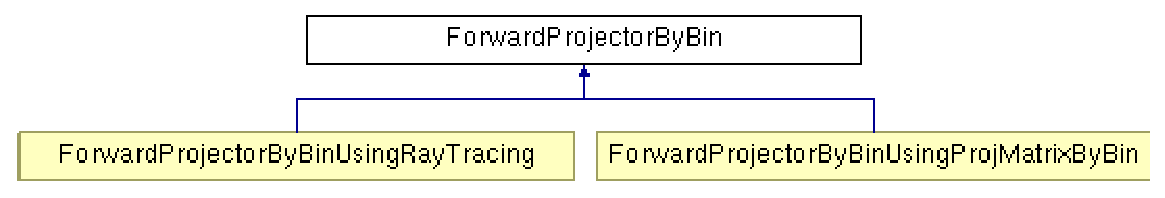
\includegraphics[bb = 0 0 543 79, scale=0.52]{graphics/STIR-developers-overviewFig10}
\caption{Forward projectors}
\end{center}
\end{figure}
This hierarchy is uses the registry mechanism discussed in section 
\ref{sect:registries}.

\subsubsection{
BackProjectorByBin hierarchy}

This is very similar to the previous section. We provide two 
derived classes of \textit{BackProjectorByBin}: 
\begin{itemize}
\item 
\textit{BackProjectorByBinUsingInterpolation} computes the $P_{bv}$ 
elements via interpolation between the projection data for the 
LOR through the centre of the voxel. We have two different interpolation 
mechanisms (linear, and piece-wise linear) as discussed in [Par4.1].
\item 
\textit{BackProjectorByBinUsingProjMatrix} performs back projection 
for any \textit{ProjMatrixByBin}. 
\end{itemize}

\begin{figure}[htbp]
\begin{center}
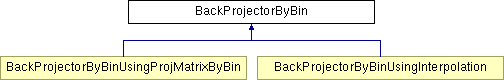
\includegraphics[bb = 0 0 503 79, scale=0.52]{graphics/STIR-developers-overviewFig11}
\caption{Back projectors}
\end{center}
\end{figure}

This hierarchy is uses the registry mechanism discussed in section 
\ref{sect:registries}.

\subsubsection{
ProjMatrixByBin hierarchy}

This is a base class for row-wise access to the projection matrix $P_{bv}$. 
This class provides 2 essential mechanisms aside from the virtual 
functions that will be used to get the row of the matrix:
\begin{itemize}
\item 
It can cache the elements of the projection matrix. This caching 
is obviously useful if you can store the part of the matrix that 
you need in memory (for instance, a slave might not need the 
whole matrix). However, even if you cannot store the whole matrix, 
most algorithms need access to a subset of these elements more 
than once (for instance, OSEM would need them for forward projecting 
and for back projecting). Caching can be disabled.
\item 
The application of symmetries is provided at base-class level: 
the derived classes do not have to bother about this, and can 
concentrate on computing the 'independent' part of $P_{bv}$. 
\end{itemize}


At the moment, we have three derived classes:
\begin{itemize}
\item 
\texttt{ProjMatrixByBinUsingRayTracing} uses essentially the same 
(although more flexible) implementation as the on-the-fly \texttt{ForwardProjectorByBinUsingRayTracing}, but 
returns the row of the projection matrix. However, because symmetries 
are not handled 'in-line', and elements need to be stored, using 
a \texttt{ProjMatrixByBinUsingRayTracing} object for forward projection 
is in some cases not as efficient as using \texttt{ForwardProjectorByBinUsingRayTracing}.
\item
\texttt{ProjMatrixByBinUsingInterpolation} implements the same as
\texttt{BackProjectorByBinUsingInterpolation}, but is much slower to initialise.
\item 
\texttt{ProjMatrixByBinFromFile} handles the case where the projection 
matrix is stored on disk [not distributed yet]. Because of the 
support provided by \texttt{ProjMatrixByBin}, only the 'independent' 
part of the projection matrix needs to be stored. Our current 
implementation does not yet provide a very compact format for 
storing the elements (although they are of course stored sparsely).
\end{itemize}

\begin{figure}[htbp]
\begin{center}
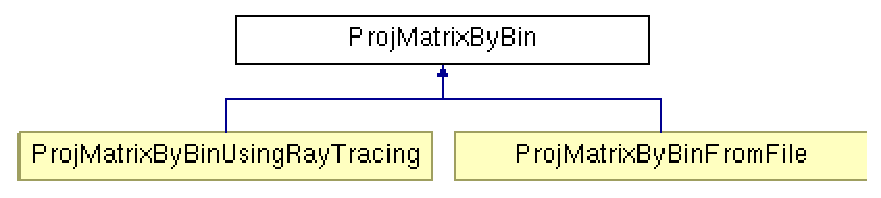
\includegraphics[bb = 0 0 407 79, scale=0.52]{graphics/STIR-developers-overviewFig12}
\caption{Projection matrix classes}
\end{center}
\end{figure}

This hierarchy uses the registry mechanism discussed in section 
\ref{sect:registries}.


\subsubsection{
ProjMatrixElementsForOneBin }

This class provides sparse storage for a row of the projection 
matrix. It has methods to access the data using an STL-style 
iterator (which is essentially a generalised pointer). This means 
that the actual way to store the data is hidden from the user. 
In principle, this format could be very compact, or alternatively 
very efficient. At the moment, we provide a format that is somewhere 
in between. For instance, image indices are not stored incrementally, 
as although it would allow very compact storage, it is detrimental 
for speed.

\subsection{Objective functions}
Many iterative (reconstruction) algorithms can be formulated in terms
of an objective function, which is the algorithms tries to 
maximise (or minimise). Since STIR 2.0, this is implemented
as a class hierarchy based on \texttt{GeneralisedObjectiveFunction},
where we use the convention that the objective function is maximised. 

Some iterative algorithms use an 'objective function' only in a 
loose sense. They might for instance allow generalisations 
which no longer optimise a function. For example in the case
of EMML with non-matching forward and back projectors, the 'gradient' 
that is computed is generally not the gradient of the
log-likelihood that corresponds to the forward projector.
However, one hopes that it still points towards the optimum.
The corresponding objective function is implemented in the class\\
\texttt{PoissonLogLikelihoodWithLinearModelForMeanAndProjData}.

There can be different objective function that use common operations.
For instance, the objective function could implement a least squares
criterion, or a Poisson log-likelihood. Both of these have a model
for the mean of the measured data (given an image). Generally speaking,
STIR implements those common operations using a separate class.
As an example, projection operations are implemented via a pointer to a 
\texttt{ProjectorByBinPair}, which in itself is a small
class hierarchy using either a \texttt{ProjMatrixByBin} object, 
or a \texttt{ForwardProjectorByBin} and \texttt{BackProjectorByBin} pair.

Often, one includes a penalty (or prior) in the objective function
(see doxygen documentation for the class \texttt{GeneralisedPrior}).
The penalty is expected to be a function that increases with higher 
penalty, so it will be \textit{subtracted}
from the unregularised case.

See the doxygen documentation \texttt{GeneralisedObjectiveFunction} for
more details.

\subsection{
Reconstruction classes}

The final ingredient for performing reconstructions is the reconstruction 
algorithm itself. We also have a hierarchy for this, as many 
iterative algorithms are similar, and differ only in some minor 
steps. We do not discuss the actual 'leaves' of the Reconstruction 
tree here.
\\
The tree starts at the abstract \texttt{Reconstruction} base class. Classes 
ending in ``\textit{Reconstruction}'' are abstract base classes for 
a family of algorithms. Classes including the name of an algorithm 
are concrete ones whose principal purpose is to implement the 
reconstruction method of the algorithm. 

Certain algorithms will only work with particular objective functions,
while others (such as gradient ascent) might work with arbitrary
objective functions.

This arrangement gives the users 
of the library a flexible range of implementation choices, allowing 
them to experiment with new algorithms and new variations of 
old ones with minimal coding effort.

The \texttt{Reconstruction} hierarchy is (since STIR 2.0) templated in 
\texttt{TargetT}. This is the type of the output, i.e. normally
the image type. Templating this type gives flexibility to have
different output-types, such as parametric images or even 
normalisation factors.

\section{
Parsing from text files (or strings)\label{sect:parsing}}
Many STIR classes are based on the \texttt{ParsingObject} class, and hence 
are able to
\begin{itemize}
\item 
ask the parameters to the user interactively
\item 
read the parameters from an Interfile-style file
\item 
return parameter info such that an Interfile-style input file 
can be created from the current set of parameters.
\end{itemize}

In the simplest case, the only thing you need to do is to add the variables
and keywords to the keymap. All functionality will then follow. See the
following example.

\begin{verbatim}
  class A : public ParsingObject
  {
    private:
    typedef ParsingObject base_type;

    int number; float a;

    void initialise_keymap()
    {
      base_type::initialise_keymap();
      this->parser.add_start_key("My Class Parameters");
      this->parser.add_key("number", &number);
      this->parser.add_key("width", &a);
      this->parser.add_stop_key("END My Class Parameters");
    }

    void set_defaults()
    {
      base_type::set_defaults();
      // specify defaults for the parameters in case they are not set.
      number = 1;
      a = 2.4F;
    }
  };

  int main(int argc, char **argv)
  {
    A a;
    // parse a file (first argument on the command line)
    a.parse(argv[1]);
    // list them back to cout
    std::cout << a.parameter_info();
    return EXIT_SUCCESS;
  }
\end{verbatim}

Check the doxygen documentation for
\texttt{ParsingObject}.

\section{
IO \label{sect:IO}}

\subsection{Images}
For images, output file formats and (since version 2.0) input file format are represented 
by objects as well, as instantiations of classes derived from 
\texttt{OutputFileFormat} and \texttt{InputFileFormat} respectively. All of
the file formats supported by STIR are stored in registries (see section \ref{sect:registries}).

Currently recommended way to read an image is as follows:
\begin{verbatim}
    typedef DiscretisedDensity<3,float> DataType ;
    std::auto_ptr<DataType> density_aptr = read_from_file<DataType>(filename);
\end{verbatim}
You will have to include \texttt{stir/IO/read\_from\_file.h} for this to work. The function
\texttt{read\_from\_file} will open the file, read an initial block of data, check
if that corresponds to the signature of any of the file formats in the
default registry, and use the first matching file format to read the data.

For output, you can use
\begin{verbatim}
   write_to_file(filename, density);
\end{verbatim}
You will have to include \texttt{stir/IO/write\_to\_file.h} for this to work. This
will write using the default output file format and is equivalent to the following:
\begin{verbatim}
    typedef DiscretisedDensity<3,float> DataType ;
    shared_ptr<OutputFileFormat<DataType > output_format_sptr =
       OutputFileFormat<DataType >::default_sptr();
   output_format_sptr->write_to_file(filename, density);
\end{verbatim}
You will have to include \texttt{stir/IO/OutputFileFormat.h} for this to work.
Currently, the default output file format in STIR is Interfile (see the User's Guide).

At present, STIR does not provide a way to open an image file for reading and writing.
Patient/study information etc is currently ignored. More dangerously, image orientation
as well.

It is relatively straightforward to add a new file format by deriving a new class
from \texttt{InputFileFormat} (for input), and adding that to the default registry
(see section \ref{sect:registries} for more details).

\subsection{Numerical arrays}
There are some functions to read/write numerical vectors/arrays from
file. Check \texttt{stir/IO/read\_data.h} (and \texttt{write\_data.h}) for
binary IO, and \texttt{stir/stream.h} for text-based IO.

\subsection{Projection data}
At present, there is no registry yet for file formats of projection data. For reading, use
\begin{verbatim}
   shared_ptr<ProjData> proj_data_sptr = ProjData::read_from_file(filename);
\end{verbatim}
This has an optional argument for read/write access to the file.

For writing, you could use
\begin{verbatim}
   ProjDataInterfile proj_data(proj_data_info_sptr, filename);
\end{verbatim}
We currently have no easy way to copy all data across from one \texttt{ProjData}
object to another. You will have to write an explicit loop over segments.

\subsection{Dynamic or gated data}
STIR 2.0 does not provide any direct facilities for reading 4D data (aside from
the ECAT conversion utilities). Basic support should come in version 2.1.
In the mean time, there is some preliminary functionality via the 
\texttt{TimeFrameDefinitions} class and the \texttt{get\_time\_frame\_info}
utility.


\section{
Using class hierarchies \label{sect:classhierarchies}}

The main strength of object-oriented programming is that you 
can write code that is as generic as possible\footnote{In C++, 
another very powerful way to write generic code are templates,
see section \ref{ssect:AdvancedCppFeatures}.}. In STIR, 
we have tried to use this feature as much as possible (although 
there are still remaining generalisations to be implemented). 
This works by having a base class and a bunch of derived classes. 
Examples of class hierarchies are given above. The question is 
however how you use these hierarchies. Some attempt is given 
here to answer this, but of course, for serious work, you really 
should read a good C++ book.\\
We will use the DiscretisedDensity hierarchy as an example, but 
the same holds for nearly all other hierarchies in STIR (or indeed 
C++). In addition, you will see some templates being used.\\
\textbf{Rule 1}: You should try to write your code using the type 
of the base-class. If this is not possible, use a class as close 
to the base-class as you can.\\
\textbf{Example}: If you have a function that manipulates images, 
write it in terms of DiscretisedDensity, not of VoxelsOnCartesianGrid.\\
\textbf{Rule 2}: Pass references or smart pointers as arguments of 
functions. Use references if you can (such that your code would 
work for any type of pointer). Never (or almost never) return 
references, but return smart pointers (or a const pointer to 
an object that is guaranteed to stay alive long enough).\\
\textbf{Example}:

\begin{verbatim}
template <int num_dimensions, typename elemT> 
shared_ptr< DiscretisedDensity<num_dimensions, elemT> >
do_something(const DiscretisedDensity<num_dimensions, elemT>& density1,
             const DiscretisedDensity<num_dimensions, elemT>& density2);
\end{verbatim}


This is necessary, as you generally cannot construct an object 
of the type of the base-class. Similarly, it is impossible to 
copy an object of a base-class. This is solved by using the \textit{virtual 
copy constructor} idiom:

\begin{verbatim}
shared_ptr< DiscretisedDensity<3,float> > new_density_sptr(density.clone());
\end{verbatim}

This constructs an object of the same type as the given density.\\
Of course, many functions do need to know the actual type of 
the parameters, either because they can work with only one type 
(for instance, ForwardProjectorByBinUsingRayTracing handles only 
VoxelsOnCartesianGrid), or because the processing will be different 
for different types. This can be solved by using C++ Run Time 
Type Information (RTTI), preferably in the form of dynamic\_cast.

\begin{verbatim}
template <typename elemT> 
void f(DiscretisedDensity<3, elemT>& density)
{
  VoxelsOnCartesianGrid<elemT> * voxels_ptr =
     dynamic_cast< VoxelsOnCartesianGrid<elemT> * > (&density);
  if (voxels_ptr == NULL)
     error("f: can only handle images of type VoxelsOnCartesianGrid\n");
  ...
}
\end{verbatim}


Note that \texttt{dynamic\_cast} of pointers allows easy checking if the 
types matched. When using references, a non-matching type will 
cause an exception to be thrown. There currently is no code in 
STIR using/catching exceptions, so if you do not catch the exception 
yourself, your program will abort mysteriously.


\section{
Registries of classes \label{sect:registries}}

Several class hierarchies in STIR keep a registry of all \textit{leaf} 
derived classes (i.e. classes at the end of the hierarchy). This 
registry allows the user to select \textit{at run-time} which image 
processor, projector, matrix, output file format etc. (s)he 
wants to use. It is fairly easy to add your own leaf class to 
the hierarchy such that it will be added to the registry. How 
to do this is briefly described here, but see the doxygen 
documentation of classes \texttt{RegisteredObject} and \texttt{RegisteredParsingObject}
and the example below. 

The recommended way to add your own class (as always) is to take 
a look at an existing leaf in the hierarchy, copy the files and 
change what you need. Also make sure you new class gets linked 
in by adding it to one of existing \textbf{*registries.cxx} files, although
it is probably better to put your own additions in separate files
such that you can easily import a new version of STIR. 
See section \ref{sect:extendingSTIR} for information on how to do that.

\subsection{How does the STIR implementation of registries work?}
The \texttt{RegisteredObject} class takes care of finding your class etc, but it
will only do that if you have registered your own class. In an attempt to 
avoid having to do this explicitly, we currently use the following scheme:
\begin{itemize}
\item creating a variable of type \texttt{yourClass::RegisterIt} will add \textit{yourClass}
to the registry as long as this variable persists.
\item we put that variable in a separate source file and declare it static. This means it
will be ``initialised'' (\textit{i.e.} its constructor will be called, which actually does the
registration) before the main program starts.
\item the special source file needs to be added explicitly to the list of files to link with\footnote{
If the file is added to a library, many linkers will think that it only contains variables which are
not referenced by anything else, so will discard it from the linking, and hence the relevant 
constructor will never be called.}. This is currently done by adding the file to the 
\texttt{STIR\_REGISTRIES} CMake variable.
\end{itemize}

\section{
Extending STIR with your own files \label{sect:extendingSTIR}}

If you want to add your own files to the libraries, or have your 
own main programs, you can of course set-up your own directory 
and
\begin{itemize}
\item 
make sure that your compiler finds the STIR include files in \textbf{STIR/include}
\item 
make sure that you link with all the necessary libraries
\item 
make sure that you link with the *\_registries object files
\end{itemize}

All of this is made easier if you  \textit{installed}
STIR after you built it (\textit{i.e.} used \texttt{make install} or built the \texttt{INSTALL}
target in your IDE).

Nevertheless, wipping up your own \textbf{CMakeLists.txt} is slightly painful, and when using the
above mechanism, it is impossible for STIR to call your own routines, \textit{e.g.} if you
added your own filter or prior and want to use that during reconstruction.
For a true integration with  STIR, we provide the following alternative.

\begin{itemize}
\item Put all your files in a separate subdirectory or in \textbf{STIR/local} (the distribution 
will never contain any files in that directory). Let us call your directory 
\textbf{mySTIRext} as an example.
\item Create a file \textbf{mySTIRext/extra\_stir\_dirs.cmake} with CMake statements,
in particular a list of your subdirectories. For instance,
\begin{verbatim}
# add include directory to compiler switches
include_directories(include)

# check CMakeLists in next directories
add_subdirectory(buildblock my_buildblock)
\end{verbatim}
where \textbf{buildblock} is the name of your subdirectory and \textbf{my\_buildblock} is a name for the
sub-directory where CMake will build the files (make sure the latter is different from any
sub-directories in \textbf{STIR/src}).

\item Put in each of your subdirectories a file called \textbf{CMakeLists.txt}
which list all files you want to compile. This file have to 
be in a specific (but simple) format. The easiest way to do this 
is to copy for instance \textbf{buildblock/CMakeLists.txt}, \textbf{utilities/CMakeLists.txt}
or  \textbf{test/CMakeLists.txt} and change the list of filenames. For instance, an extra library
would be specified like this:
\begin{verbatim}
set(dir my_buildblock)
set (dir_LIB_SOURCES ${dir}_LIB_SOURCES)

set(${dir_LIB_SOURCES}
   my_source1
   my_source2
)

# declare dependencies on other STIR libraries, for instance
target_link_libraries($(dir) buildblock)

# add to list of libraries for STIR to include in linking
list(APPEND STIR_LIBRARIES $(dir))

# add source file for registries (if you have one)
list(APPEND STIR_REGISTRIES my_registry)

include(stir_lib_target)
\end{verbatim}

\item Re-run \textbf{CMake} and set the CMake variable \texttt{STIR\_LOCAL} to the directory where your
\textbf{extra\_stir\_dirs.cmake} file (\textit{i.e.} \textbf{mySTIRext} in this example),
the result will be that, when you (re-)build STIR, your files will be included in 
the normal build/test process.
\end{itemize}

As discussed in section \ref{sect:registries}, if you implement a projector, filter
or similar, you will need to add it to its relevant registry
such that normal STIR utilities can use it at run-time.
As an example, let us say you have written a class that implements
a different output fileformat. You could create a new file \textbf{my\_registry.cxx} with
content like this
\begin{verbatim}
#include "myOutputFileFormat.h"
static myOutputFileFormat::RegisterIt dummy1;
\end{verbatim}
If you add that to the \texttt{STIR\_REGISTRIES} variable in your \textbf{CMakeListst.txt}
as above, everything should work as expected.


\section{
Conclusion}

In many cases, a reconstruction algorithm does not have to know 
about the type of the image it gets. In our set-up this means 
it can/should be implemented in terms of a \textit{DiscretisedDensity} 
object, and \textit{ForwardProjectorByBin} and \textit{BackProjectorByBin} 
objects (or \textit{ProjMatrixByBin} object). This means that once 
for instance EM is implemented, it can be used on voxels, blobs, 
different grids etc. without having to rewrite the algorithm 
itself (of course, the projectors do depend on the actual type 
of image, so you would have to write those).\\
The STIR library allows maximal code re-use when implementing 
new functionality. Its structure and its documentation features 
make it into a unique resource for the PET/SPECT community. 

\end{document}
